\listfiles

\documentclass[11.5pt,a4paper]{article}

\usepackage{amsthm,amssymb,amsmath}
\usepackage{wasysym}
\usepackage{mathtools}

\newcommand\persiangloss[2]{#1\dotfill\lr{#2}\\}

\newcommand{\nocontentsline}[3]{}
\newcommand{\tocless}[2]{\bgroup\let\addcontentsline=\nocontentsline#1{#2}\egroup}
\usepackage[bottom]{footmisc}
\usepackage{indentfirst}

\usepackage{caption}

\usepackage{graphicx}
\usepackage{subcaption}
\usepackage{array}
\usepackage{adjustbox}
\usepackage{tablefootnote}
\usepackage{amsfonts}
\usepackage{amssymb}
\usepackage{yfonts}
\usepackage{subcaption}
\usepackage{relsize}

\usepackage[scr=euler,bb=ams]{mathalfa}

\usepackage{xcolor,colortbl}
\definecolor{Gray}{gray}{0.90}
\definecolor{LGray}{gray}{0.95}

\usepackage[pagebackref=false,colorlinks,linkcolor=blue,citecolor=magenta]{hyperref}

\usepackage[a4paper]{geometry} 
\geometry{a4paper,tmargin=3.5cm, bmargin=2.5cm, lmargin=2cm, rmargin=2.5cm, headheight=3em, headsep=1.5cm, footskip=1cm} 

\usepackage{xepersian}
\settextfont[Scale=1]{B Nazanin}
%\setlatintextfont[Scale=1]{Times New Roman}

%\settextfont[Scale=1.1]{B Zar}

%\DefaultMathsDigits
\setdigitfont{XB Zar}

\defpersianfont\titr[Scale=1]{B Titr}
%\defpersianfont\nastaliq[Scale=1.5]{IranNastaliq}
%\defpersianfont\traffic[Scale=1]{B Traffic}
%\defpersianfont\yekan[Scale=1]{B Yekan}
%\defpersianfont\traffic[Scale=1]{XB Roya}
%\defpersianfont\yekan[Scale=1]{XB Kayhan}
%%%%%%%%%%%%%%%%%%%%%%%%%%%%%%%%%%%%%%%%%%%%%%%%%%%
\usepackage{zref-perpage}
\zmakeperpage{footnote}



\begin{document}

\thispagestyle{empty}
\vspace*{-28mm}
\centerline{
\includegraphics[height=5cm]{Imgs/ceit_logo.png}}

\begin{center}
%دستوری برای کم کردن فاصله بین لوگو و خط پایین آن
\vspace{-2mm}
{\LARGE
{
دانشکده مهندسی کامپیوتر و فن‌آوری اطلاعات\\	
دانشگاه صنعتی امیرکبیر	
}
%دستوری برای تعیین فاصله بین دو خط
\\[2.1cm]
}

{\large
\textbf{گزارش تمرین دوم درس مدل‌های احتمالاتی گرافی}
\\[2cm]

استاد درس:
\\[.5cm]
{\Large
دکتر نیک‌آبادی}
\\[1.5cm]
\large 
نام دانشجو:
\\[.5cm]
{\Large
احمد اسدی}
\\[.5cm]
۹۴۱۳۱۰۹۱
\\[1.5cm]
}
%دستوری برای تعیین فاصله بین خطوط (نه دو خط) و تا وقتی که مقدار آن تغییر نکند، فاصله بین خطوط، همین مقدار است.

{\large
فروردین ۱۳۹۵
}
\end{center}

\newpage
\baselineskip=1cm
\tocless\tableofcontents

\newpage
\baselineskip=0.75cm
\pagenumbering{arabic}

%%%%%%%%%%%%%%%%%%%%%%%%%%%%%%%%%%%%%%%%%%%%%%%%%%%%%%%%%%%%%%%%%%%%%%%%%%%%%%%%%%%
\section{تقطیع با دسته‌بندی‌کننده بیز ساده}
در این قسمت، ابتدا به بررسی دسته‌بندی‌کننده بیز به عنوان عملگر تقطیع پرداخته و سپس تاثیر نویز‌ها مختلف بر نتیجه این دسته‌بندی‌کننده را بررسی می‌نماییم.
%%%%%%%%%%%%%%%%%%%%%%%%%%%%%%%%%%%%%%%%%%%%%%%%%%%%%%%%%%%%%%%%%%%%%%%%%%%%%%%%%%%
\subsection{دسته‌بندی‌کننده بیز ساده به عنوان عملگر تقطیع}
در این بخش قصد داریم، با استفاده از دسته‌بندی‌کننده بیز ساده، تصویر ورودی را به سه قطعه مختلف تقسیم نماییم. برای این منظور، تنها از مقدار سطح خاکستری نقاط تصویر به عنوان ویژگی استفاده می‌نماییم. رابطه 
\ref{eq:NB}،
به عنوان رابطه پایه این دسته‌بندی‌کننده مورد استفاده قرار می‌گیرد. در این بخش ابتدا با استفاده از روش \lr{MAP} \footnote{\lr{Maximum A Posteriori }}، 
کلاس مربوط به هر پیکسل را تخمین می‌زنیم. 
\begin{equation}
\label{eq:NB}
P(\Theta | X) = \frac{ P(\Theta,X)}{P(\Theta)}
\end{equation}
به عنوان اولین گام در این فرایند،‌ باید مدل بیز ساده را جهت تقطیع تصویر به سه قطعه مختلف، آموزش دهیم. برای آموزش این مدل، کافیست تعداد پیکسل‌ها از هر سطح خاکستری مختلف را شمارش کنیم. با توجه به این‌ که تمام پیکسل‌های تصویر آموزشی ما فقط دارای سه سطح خاکستری مختلف هستند، هر سطح خاکستری دقیقا بیانگر یک کلاس است. با این توضیح، نسبت تعداد پیکسل‌های هر سطح خاکستری به کل پیکسل‌ها برابر با $P(\Theta)$ است. برای مدل کردن احتمال توام $P(\Theta,X)$ از یک توزیع گاوسی استفاده می‌نماییم که میانگین آن برابر با سطح خاکستری کلاس مورد نظر باشد و واریانس هر سه توزیع توام (یک توزیع به ازای هر کلاس) را با هم برابر و برابر با 0.125 در نظر می‌گیریم. شکل
\ref{fig:P0XL}
توزیع احتمالی توام اولیه را که در این بخش در نظر گرفته شده است، نمایش می‌دهد. 
\begin{figure}[h]
\center
\caption{توزیع احتمالی توام کلاس‌‌های مختلف}
\label{fig:P0XL}
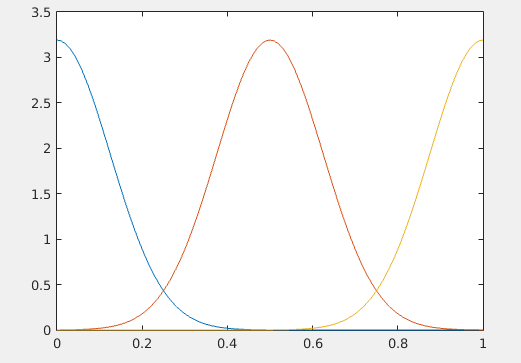
\includegraphics[scale=0.5]{Imgs/P0XL}
\end{figure}
با اعمال شرایط فوق به مدل، می‌توان مدل را طوری آموزش داد که برای تقطیع تصویر به سه سطح خاکستری مناسب باشد. این مدل روی داده‌های بدون نویز به طور دقیق عمل می‌نماید. اما در مواردی که تصویر شامل نویز باشد، بسته به قدرت نویز در هر پیکسل می‌تواند دچار خطا شود. با توجه به نمودار\ref{fig:P0XL}، پیکسل‌هایی که در اثر نویز، تغییر زیادی در سطح خاکستری آن‌ها ایجاد شده باشد، اشتباه تشخیص داده‌‌ خواهند شد. 


%%%%%%%%%%%%%%%%%%%%%%%%%%%%%%%%%%%%%%%%%%%%%%%%%%%%%%%%%%%%%%%%%%%%%%%%%%%%%%%%%%%
\subsection{تاثیر نویزهای مختلف بر عملکرد دسته‌بندی‌کننده بیز ساده}


شکل
\ref{fig:NB_Res}
نشان‌دهنده نتیجه تقطیع تصاویر با استفاده از دسته‌بندی‌کننده بیز ساده است.
همان‌طور که مشاهده می‌شود، در صورتی که قدرت نویز اعمال شده، خیلی زیاد نباشد، دسته‌بندی‌کننده قادر به دسته‌بندی صحیح تصویر است. اما در صورتی‌که نویز ورودی، قدرت زیادی داشته باشد، این دسته‌بندی‌کننده کمک زیادی به تقطیع تصویر نمی‌کند. در شکل
\ref{fig:NB_Res}
به هیستوگرام تصاویر نویزی دقت نمایید. تا جاییکه شکل این هیستوگرام شبیه به شکل 
\ref{fig:P0XL}
باشد، دسته‌بندی‌کننده به خوبی عمل می‌کند. در غیر این صورت، عمل تقطیع با مشکل روبرو می‌شود.

\begin{figure}[h]
\center
	\begin{subfigure}{.3\textwidth}
%		\center
		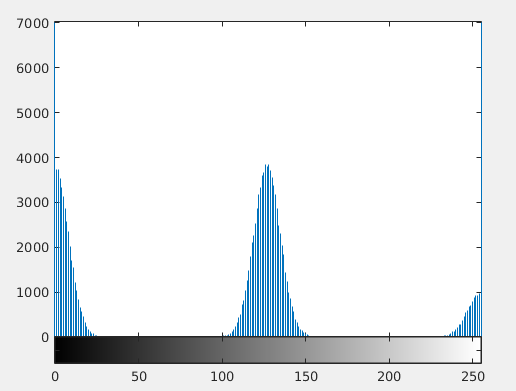
\includegraphics[scale=0.2]{Imgs/NB_S001_Hist.png}
		\caption{هیستوگرام تصویر نویزی با $\sigma=0.001$}
	\end{subfigure}
	\begin{subfigure}{.3\textwidth}
%		\center
		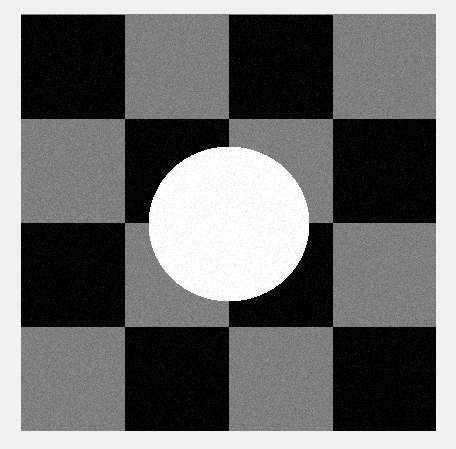
\includegraphics[scale=0.2]{Imgs/NB_S001_In.png}
		\caption{تصویر نویزی با $\sigma=0.001$}
	\end{subfigure}
	\begin{subfigure}{.3\textwidth}
%		\center
		
\includegraphics[scale=0.2]{Imgs/NB_S001_Res.png}
		\caption{نتیجه تقطیع تصویر نویزی با $\sigma=0.001$}
	\end{subfigure}

	\begin{subfigure}{.3\textwidth}
%		\center
		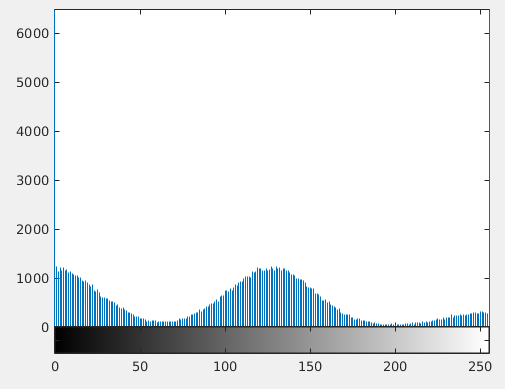
\includegraphics[scale=0.2]{Imgs/NB_S01_Hist.png}
		\caption{هیستوگرام تصویر نویزی با $\sigma=0.01$}
	\end{subfigure}
	\begin{subfigure}{.3\textwidth}
%		\center
		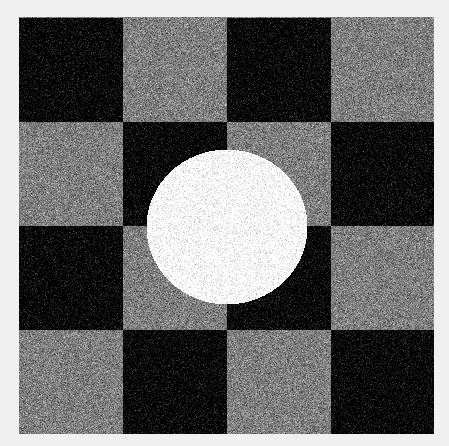
\includegraphics[scale=0.2]{Imgs/NB_S01_In.png}
		\caption{تصویر نویزی با $\sigma=0.01$}
	\end{subfigure}
	\begin{subfigure}{.3\textwidth}
%		\center
		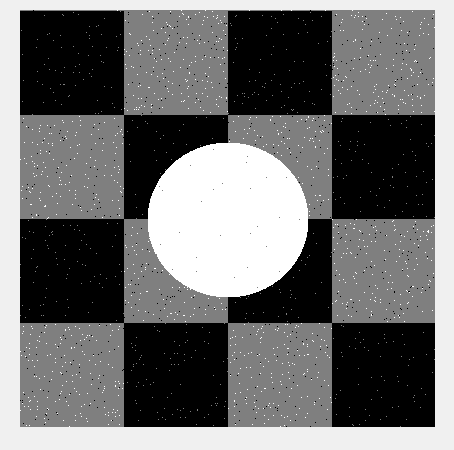
\includegraphics[scale=0.2]{Imgs/NB_S01_Res.png}
		\caption{نتیجه تقطیع تصویر نویزی با $\sigma=0.01$}
	\end{subfigure}

	\begin{subfigure}{.3\textwidth}
%		\center
		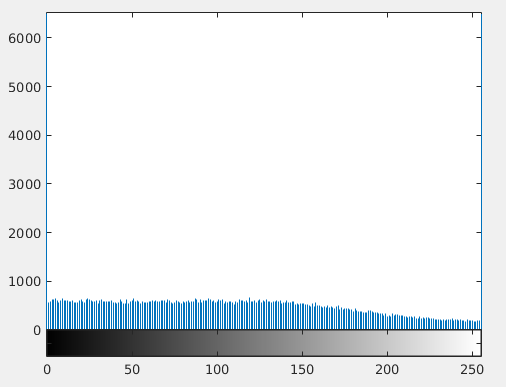
\includegraphics[scale=0.2]{Imgs/NB_S05_Hist.png}
		\caption{هیستوگرام تصویر نویزی با $\sigma=0.05$}
	\end{subfigure}
	\begin{subfigure}{.3\textwidth}
%		\center
		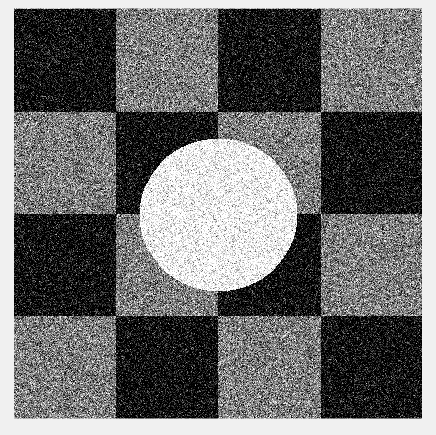
\includegraphics[scale=0.2]{Imgs/NB_S05_In.png}
		\caption{تصویر نویزی با $\sigma=0.05$}
	\end{subfigure}
	\begin{subfigure}{.3\textwidth}
%		\center
		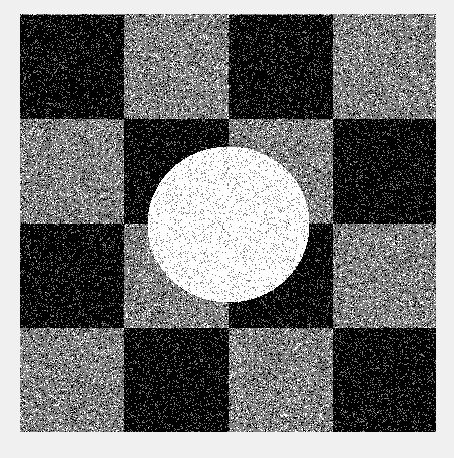
\includegraphics[scale=0.2]{Imgs/NB_S05_Res.png}
		\caption{نتیجه تقطیع تصویر نویزی با $\sigma=0.05$}
	\end{subfigure}

	\begin{subfigure}{.3\textwidth}
%		\center
		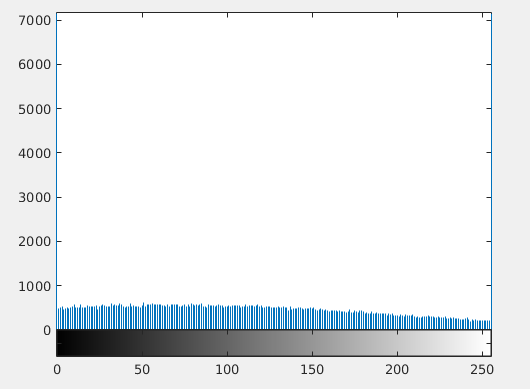
\includegraphics[scale=0.2]{Imgs/NB_S1_Hist.png}
		\caption{هیستوگرام تصویر نویزی با $\sigma=0.1$}
	\end{subfigure}
	\begin{subfigure}{.3\textwidth}
%		\center
		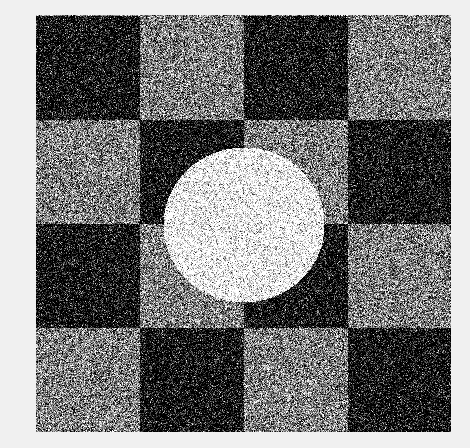
\includegraphics[scale=0.2]{Imgs/NB_S1_In.png}
		\caption{تصویر نویزی با $\sigma=0.1$}
	\end{subfigure}
	\begin{subfigure}{.3\textwidth}
%		\center
		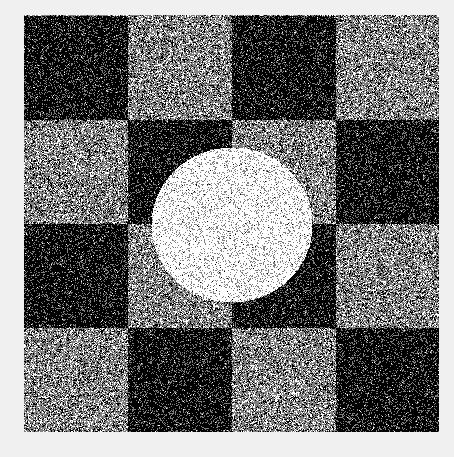
\includegraphics[scale=0.2]{Imgs/NB_S1_res.png}
		\caption{نتیجه تقطیع تصویر نویزی با $\sigma=0.1$}
	\end{subfigure}

	\begin{subfigure}{.3\textwidth}
%		\center
		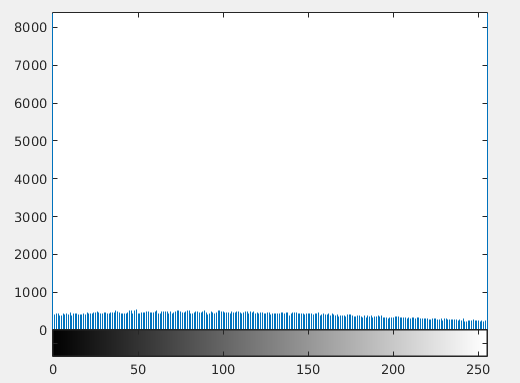
\includegraphics[scale=0.2]{Imgs/NB_S2_Hist.png}
		\caption{هیستوگرام تصویر نویزی با $\sigma=0.2$}
	\end{subfigure}
	\begin{subfigure}{.3\textwidth}
%		\center
		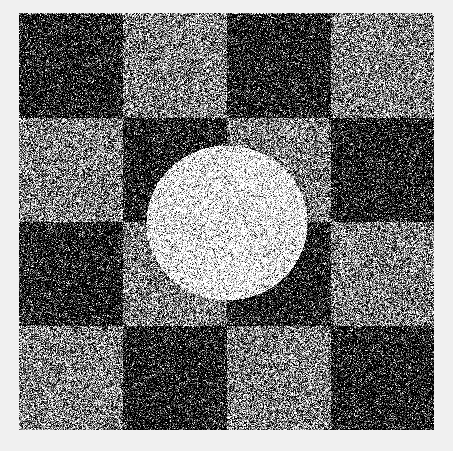
\includegraphics[scale=0.2]{Imgs/NB_S2_In.png}
		\caption{تصویر نویزی با $\sigma=0.2$}
	\end{subfigure}
	\begin{subfigure}{.3\textwidth}
%		\center
		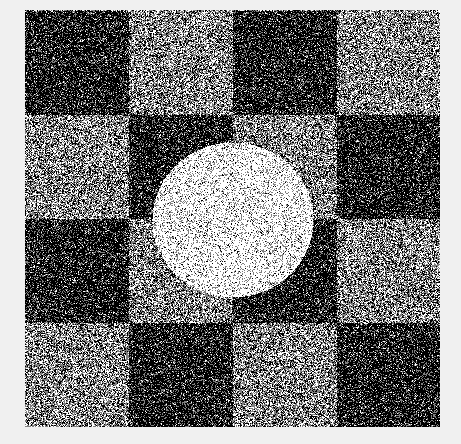
\includegraphics[scale=0.2]{Imgs/NB_S2_Res.png}
		\caption{نتیجه تقطیع تصویر نویزی با $\sigma=0.02$}
	\end{subfigure}

	\begin{subfigure}{.3\textwidth}
%		\center
		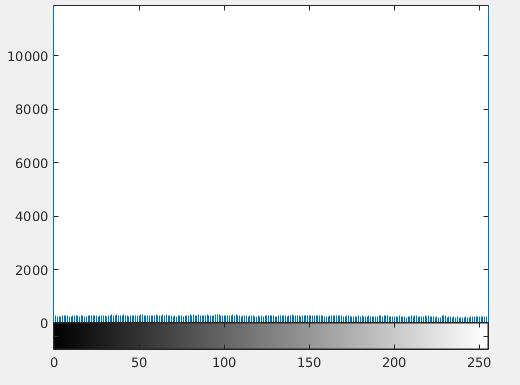
\includegraphics[scale=0.2]{Imgs/NB_S8_Hist.png}
		\caption{هیستوگرام تصویر نویزی با $\sigma=0.8$}
	\end{subfigure}
	\begin{subfigure}{.3\textwidth}
%		\center
		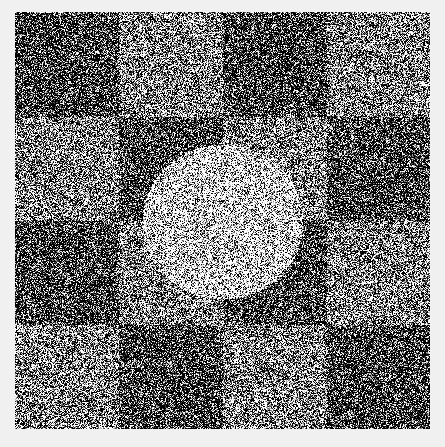
\includegraphics[scale=0.2]{Imgs/NB_S8_In.png}
		\caption{تصویر نویزی با $\sigma=0.8$}
	\end{subfigure}
	\begin{subfigure}{.3\textwidth}
%		\center
		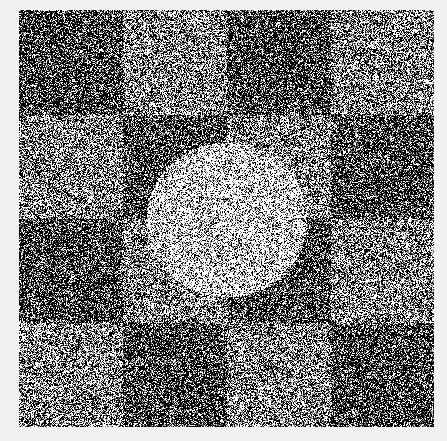
\includegraphics[scale=0.2]{Imgs/NB_S8_Res.png}
		\caption{نتیجه تقطیع تصویر نویزی با $\sigma=0.8$}
	\end{subfigure}
\caption{نتایج عملکرد دسته‌بندی‌کننده بیز ساده در تقطیع تصاویر. در تمام تصاویر  
$\mu_{noise} = 0$
}
\label{fig:NB_Res}
\end{figure} 
%%%%%%%%%%%%%%%%%%%%%%%%%%%%%%%%%%%%%%%%%%%%%%%%%%%%%%%%%%%%%%%%%%%%%%%%%%%%%%%%%%%
%%%%%%%%%%%%%%%%%%%%%%%%%%%%%%%%%%%%%%%%%%%%%%%%%%%%%%%%%%%%%%%%%%%%%%%%%%%%%%%%%%%
\section{تقطیع با استفاده از مدل میدان تصادفی مارکف }
برای بهبود عملکرد تقطیع،‌ می‌توان از مدل میدان تصادفی مارکف استفاده کرد. در این مدل علاوه بر فاکتور میزان سطح خاکستری نقاط،‌ فاکتور دیگری تحت عنوان سازگاری با نقاط همسایه، تعریف نموده و از آن در فرایند تقطیع استفاده می‌نماییم. ایده اصلی در این بخش این است که معمولا برچسب هر پیکسل، با برچسب همسایگان آن پیکسل، سازگار است. با در نظر گرفتن این فاکتور، از ایجاد نقاط یکه در تصویر که برچسب آن‌ها با برچسب همه یا بیشتر همسایگانش مغایر باشد جلوگیری می‌کنیم.\\
در ادامه،‌ ابتدا به بیان مدل پرداخته و روش اجرای الگوریتم را توضیح خواهیم داد. سپس به بررسی پارامترهای مدل از جمله میزان اهمیت یکپارچگی برچسب‌ها نسبت به سطح خاکستری پیکسل‌ها،‌ نحوه تغییر دما، میزان نویز موجود در تصویر، نوع همسایگی و مقداردهی دستی اولیه برخی پیکسل‌ها را مورد بررسی قرار خواهیم داد.

\subsection{بررسی مدل}
اگر فاکتور اول را برابر با توزیع احتمال توام برچسب هر نقطه و سطح خاکستری آن مطابق با رابطه
\ref{eq:firstFact}
 در نظر بگیریم و فاکتور دوم را مطابق با رابطه
\ref{eq:IntegFact}
تعریف کنیم، رابطه 
\ref{eq:MRF}
بیان‌کننده مدل مورد استفاده در این بخش خواهد بود.
\begin{equation}
\label{eq:firstFact}
\Phi_{i}(X_i,\Theta) = PDF(X_i;\mu_{\Theta} , \sigma_{\Theta}) 
\end{equation}
\begin{equation}
\label{eq:IntegFact}
\Phi_{ij}(X_i,X_j) = 
	\left\{
		\begin{array}{ll}
			1	&  \Theta_{X_i} = \Theta_{X_j} \\
			-1	&  \Theta_{X_i} \neq \Theta_{X_j}
		\end{array}
	\right.
\end{equation}
\begin{equation}
\label{eq:MRF}
P(X_1, X_2, \cdots, X_n, \Theta) = \frac{1}{Z} \mathlarger{\mathlarger{(\Pi_{i=1}^n\Pi_{j \in Neighbours(X_i)} \Phi_{ij}) \cdot \Pi_{i=1}^n \Phi_i}}
\end{equation}

برای تشخیص برچسب هر پیکسل در این حالت، باید $\Theta$ را طوری پیدا کنیم که رابطه 
\ref{eq:MRF}
بیشینه شود. برای بدست آوردن این مقدار،‌ تابع آرا را به شکل رابطه 
\ref{eq:votes}
تعریف می‌کنیم و با استفاده از روش شبیه‌سازی تابکاری\footnote{\lr{Simulated Annealing}}  پارامتر بهینه $\Theta^*$ را محاسبه می‌نماییم. 
\begin{equation}
\label{eq:votes}
V = \mathlarger{\mathlarger{\mathlarger{\Sigma}}}_{i=1}^n ((1-\beta) \Phi_i(X_i,\Theta) + \Sigma_{j \in Neighbours(X_i)} \beta \Phi_{ij}(X_i, X_j))
\end{equation}

با توجه به این که محاسبه تابع آرا برای کل تصویر زمان‌بر است، به جای محاسبه مقدار کل تابع آرا در هر مرحله از الگوریتم شبیه‌سازی تابکاری، مستقیما میزان اختلاف ایجاد شده در تابع آرا به ازای تغییر برچسب پیکسل $r$ ام را محاسبه می‌کنیم. رابطه
\ref{eq:deltaV}
میزان اختلاف تابع آرا به ازای تغییر برچسب پیکسل $r$ام، محاسبه می‌نماید.
\textbf{
 با اعمال این روش، سرعت اجرای الگوریتم به صورت چشم‌گیری افزایش یافت.
}

\begin{equation}
\label{eq:deltaV}
\Delta V = (1-\beta)(\Phi_{r}(X_r, \Theta_r^{new}) - \Phi_{r}(X_r, \Theta_r^{old})) + 2\beta  \mathlarger{\mathlarger{\Sigma}}_{j \in Neighbours(X_r)} (\Phi_{rj}^{new}(X_r,X_j) - \Phi_{rj}^{old}(X_r,X_j))
\end{equation}

در پیاده‌سازی الگوریتم شبیه‌سازی تابکاری، از پارامتر دیگری تحت عنوان نرخ تغییر در تکرار، علاوه بر پارامترهای ذکر شده استفاده شده است. این پارامتر مشخص می‌کند در هر تکرار الگوریتم چه نرخی از تصویر را باید تغییر دهیم. تغییرات به شکل نقطه به نقطه اعمال می‌شوند و تصمیم‌گیری برای پذیرش تغییرات بعد از اعمال هر تغییر صورت می‌گیرد. پس از اعمال تمام تغییرات مجاز در یک تکرار، تمامی پارامترها از جمله نرخ تغییر در تکرار به شکل خطی تغییر می‌کنند. رابطه
\ref{eq:MR}
نحوه کاهش نرخ تغییرات در هر تکرار را نمایش می‌دهد.
\begin{equation}
\label{eq:MR}
\xi =  \xi_{init} + \alpha k
\end{equation}
\\
شکل
\ref{fig:MRF_NB_Comp}
خروجی مدل مارکف را با خروجی مدل بیز ساده برای یک ورودی نویزی نمایش ‌می‌دهد. همان‌طور که ملاحظه می‌شود، عملکرد مدل میدان تصادفی مارکف در مقایسه با نویز بسیار بهتر از عملکرد مدل بیز ساده است.
همان‌طور که مشاهده می‌شود، در خروجی مدل میدان تصادفی مارکف خطاهایی وجود دارد که با ادامه دادن الگوریتم این خطاها هم از بین خواهند رفت اما به دلیل کم بودن دما در این مراحل، تعداد تکرار برای حذف این خطاها زیاد است. بنابراین، الگوریتم را در مرحله دهم متوقف کردیم.
\begin{figure}[h]
\center
	\begin{subfigure}{0.3\textwidth}
		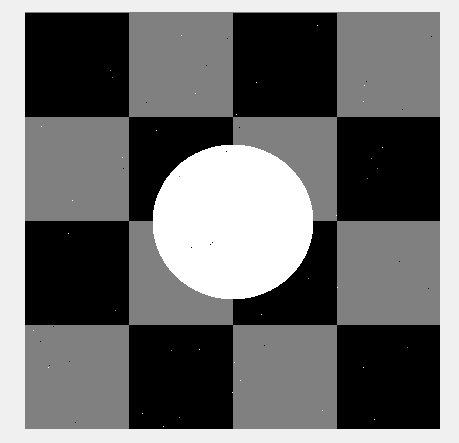
\includegraphics[scale=0.3]{Imgs/MRF_Iter10_Final.png}
		\caption{خروجی مدل مارکف در تکرار 10}
	\end{subfigure}
	\begin{subfigure}{0.3\textwidth}
		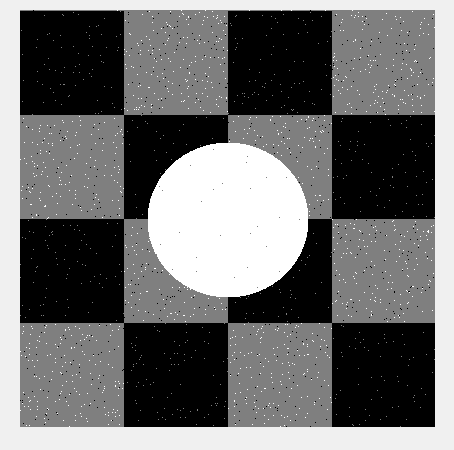
\includegraphics[scale=0.3]{Imgs/NB_S01_Res.png}
		\caption{خروجی مدل بیز ساده}
	\end{subfigure}
	\begin{subfigure}{0.3\textwidth}
		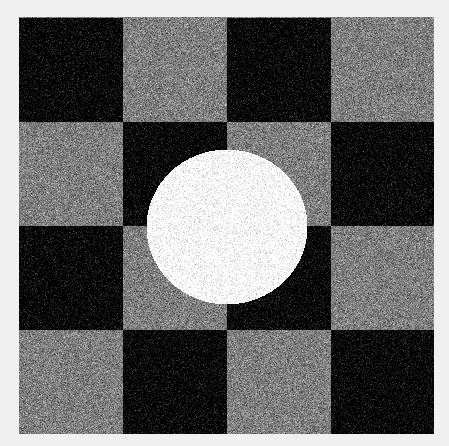
\includegraphics[scale=0.3]{Imgs/NB_S01_In.png}
		\caption{تصویر ورودی با نویز گاوسی و $\sigma = 0.01$}
	\end{subfigure}
\caption{مقایسه خروجی‌ مدل‌های مارکف و بیز ساده}
\label{fig:MRF_NB_Comp}
\end{figure}



%%%%%%%%%%%%%%%%%%%%%%%%%%%%%%%%%%%%%%%%%%%%%%%%%%%%%%%%%%%%%%%%%%%%%%%%%%%%%%%%%%%
\subsection{تاثیر اهمیت یکپارچگی برچسب‌ها نسبت به سطح خاکستری}
در رابطه 
\ref{eq:deltaV}،
پارامتر $\beta$ تنظیم‌کننده میزان اهمیت فاکتور یکپارچگی برچسب‌ها نسبت به فاکتور سطح خاکستری است. هرچه این مقدار بزرگتر باشد، تاثیر این فاکتور از فاکتور سطح خاکستری بیشتر می‌شود. اگر مقدار این پارامتر به صفر برسد، مدل ارائه شده تبدیل به مدل بیز ساده که در قسمت قبل معرفی شد، می‌شود. 
\\

روش‌های مختلفی برای پیداکردن مقدار بهینه برای این پارامتر وجود دارد. ما در این پروژه،‌ مقدار این پارامتر را به طور خطی مطابق با رابطه
\ref{eq:betaLine}
تغییر می‌دهیم.
در این رابطه،‌ $\alpha$ شیب خط افزایشی،‌ $k$ شماره مرحله و $\beta_{init}$ مقدار اولیه $\beta$ است.
\begin{equation}
\label{eq:betaLine}
\beta = \beta_{init} + \alpha k
\end{equation}

مقدار اولیه $\beta_{init}$ را صفر قرار می‌دهیم تا در مرحله اول، مدل شبیه مدل بیز عمل کند. به این طریق، الگوریتم به سرعت به حالتی نزدیک به حالت بهینه نزدیک می‌شود. \textbf{اعمال این روش، تاثیر بسزایی در افزایش سرعت همگرایی الگوریتم ایجاد کرد.} به این طریق در اولین تکرار، خروجی الگوریتم شبیه خروجی دسته‌بندی‌کننده بیز ساده می‌شود. با تکرار مراحل بعدی، گام به گام سعی در حذف نویز در تصویر نهایی می‌کنیم. با افزایش گام به گام این پارامتر، اهمیت برچسب پیکسل‌های همسایه،‌ بیشتر می‌شود و پیکسل‌هایی که به طور یکه در یک همسایگی دارای برچسبی متفاوت نسبت به همسایگان خود هستند، تصحیح می‌شوند. این مراحل به بهبود عملکرد مدل کمک زیادی می‌کنند.
\\
شکل 
\ref{fig:Beta}
تاثیر پارامتر $\beta$ را بر عملکرد الگوریتم نمایش می‌دهد.
نویز تصویر در همه مراحل این آزمایش به شکل گاوسی و با $\sigma=0.1$ اعمال شده است. همان‌طور که در شکل مشاهده می‌شود، مقادیر پایین برای پارامتر $\beta$ قدرت الگوریتم را در رفع نویز، کاهش می‌دهد.
از طرفی، افزایش بیش از حد مقدار این پارامتر هم، با غلبه بر مقدار فاکتور اول (سطح خاکستری نقطه) منجر به افزایش خطا و کاهش کارایی الگوریتم می‌شود. بهترین روش ممکن برای کنترل الگوریتم و بالا بردن سرعت، افزایش تدریجی این پارامتر به صورت خطی است.
\begin{figure}[h]
\center
	\begin{subfigure}{0.3\textwidth}
	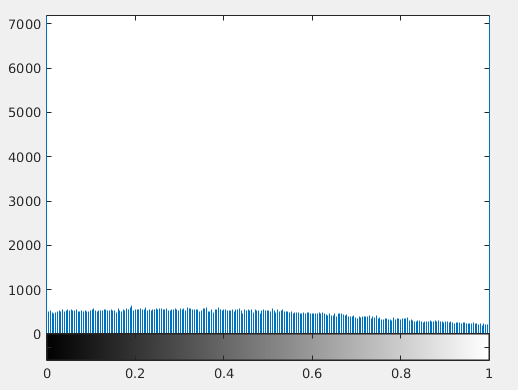
\includegraphics[scale=0.3]{Imgs/MRF_S1_Hist.png}
	\caption{هیستوگرام تصویر نویزی با $\sigma=0.1$}
	\end{subfigure}
	\begin{subfigure}{0.3\textwidth}
	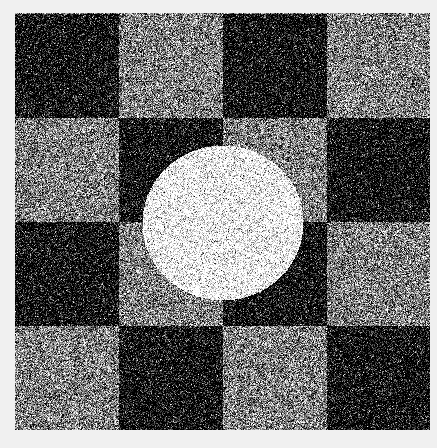
\includegraphics[scale=0.3]{Imgs/MRF_S1_In.png}
	\caption{تصویر نویزی ورودی با $\sigma=0.1$}
	\end{subfigure}
	\begin{subfigure}{0.3\textwidth}
	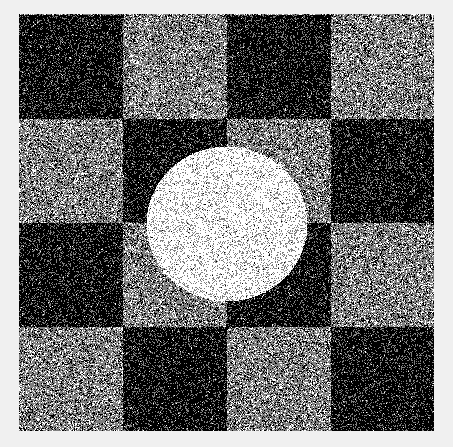
\includegraphics[scale=0.3]{Imgs/MRF_S1_Beta05_Res.png}
	\caption{خروجی الگوریتم با $\beta=0.05$}
	\end{subfigure}
	\begin{subfigure}{0.3\textwidth}
	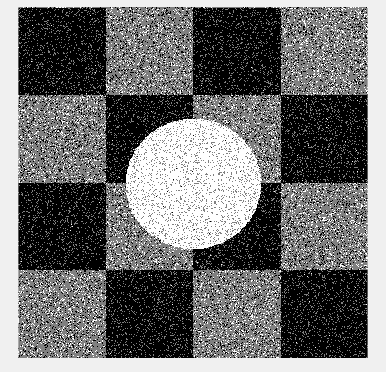
\includegraphics[scale=0.35]{Imgs/MRF_S1_Beta2_Res.png}
	\caption{خروجی الگوریتم با $\beta=0.2$}
	\end{subfigure}
	\begin{subfigure}{0.3\textwidth}
	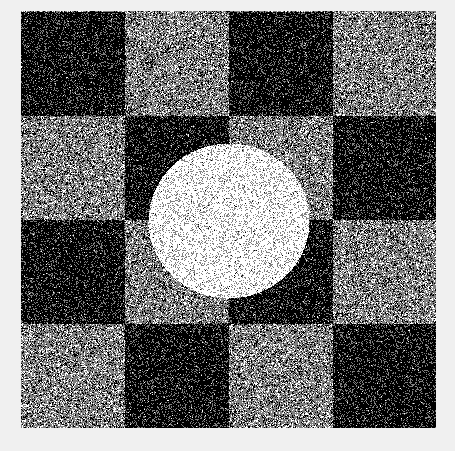
\includegraphics[scale=0.3]{Imgs/MRF_S1_Beta8_Res.png}
	\caption{خروجی الگوریتم با $\beta=0.8$}
	\end{subfigure}
	\begin{subfigure}{0.3\textwidth}
	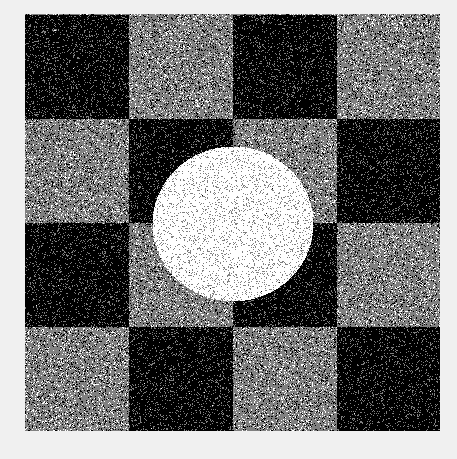
\includegraphics[scale=0.3]{Imgs/MRF_S1_BetaV_Res.png}
	\caption{خروجی الگوریتم با $\beta$ متغیر}
	\end{subfigure}
	
\caption{مقایسه تاثیر پارامتر  $\beta$}
\label{fig:Beta}
\end{figure}

%%%%%%%%%%%%%%%%%%%%%%%%%%%%%%%%%%%%%%%%%%%%%%%%%%%%%%%%%%%%%%%%%%%%%%%%%%%%%%%%%%%
\subsection{نحوه تغییر دما}
در این قسمت، دو مرحله تغییر دمای مختلف را مورد بررسی قرار می‌دهیم. در روش اول، دمای سیستم را به طور خطی کاهش می‌دهیم تا به یک حد آستانه‌ای برسد. در روش دوم، دما را مطابق با یک نمودار نمایی تغییر می‌دهیم .
در روش اول، دما مطابق با رابطه 
\ref{eq:TLin}
و در روش دوم،‌ مطابق با رابطه
\ref{eq:TExp} 
تغییر می‌کند. در هر دو رابطه، $k$ شماره مرحله و $\alpha > 0$ و $\gamma > 0$ مقادیر ثابت هستند.

\begin{equation}
\label{eq:TLin}
T = T_{init} + \alpha k
\end{equation}
\begin{equation}
\label{eq:TExp}
T = \frac{1}{\sqrt{2\pi}} \cdot e \cdot (-0.05 k^2) + 10
\end{equation}

در رابطه \ref{eq:TLin}، دما به طور یکنواخت و خطی،‌ کاهش می‌یابد. زمانی که دما زیاد است، به الگوریتم بیشتر اجازه می‌دهیم تا پارامتر غیر بهینه را انتخاب نماید و رفتار تصادفی الگوریتم شدید است. اما به مرور زمان و به طور یکنواخت،‌ این اجازه کمتر می‌شود و در مراحل انتهایی الگوریتم، رفتار تصادفی به حداقل ممکن خود می‌رسد و الگورتم، فقط در جهت بهبود نتیجه حرکت می‌کند.
\\
در رابطه \ref{eq:TExp}، دما به طور نمایی کاهش می‌یابد به طوری‌که در تعداد زیادی از مراحل،‌ دما زیاد است و رفتار تصادفی الگوریتم شدید است. در اواخر الگوریتم،‌ دما با شیب زیادی کاهش می‌یابد و الگوریتم زمان کافی برای بهبود پاسخ نخواهد داشت.\\
شکل 
\ref{fig:T}
نتایج الگوریتم به ازای اجرای هر دو نحوه تغییر دما را نمایش می‌دهد. همان‌طور که انتظار می‌رود، بهترین عملکرد با تغییر دمای خطی بدست‌ آمده است.
\begin{figure}[h]
\center
	\begin{subfigure}{0.4\textwidth}
	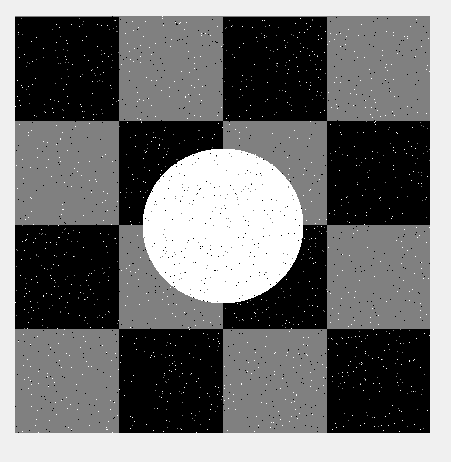
\includegraphics[scale=0.3]{Imgs/MRF_Iter4_TLin.png}
	\caption{تغییر دما به صورت خطی. نتیجه در تکرار چهارم}
	\end{subfigure}
	\begin{subfigure}{0.4\textwidth}
	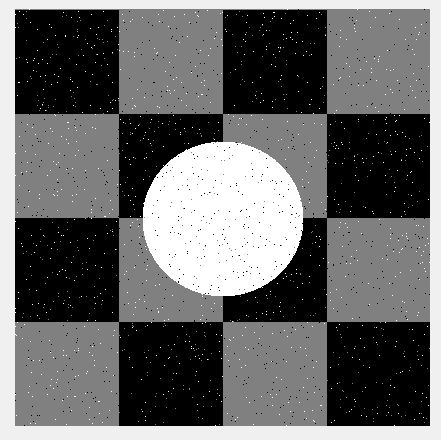
\includegraphics[scale=0.3]{Imgs/MRF_Iter4_TExp.png}
	\caption{تغییر دما به صورت نمایی. نتیجه در تکرار چهارم}
	\end{subfigure}	
\caption{مقایسه تاثیر نحوه تغییر دما با تصویر ورودی بدون نویز}
\label{fig:T}
\end{figure}


%%%%%%%%%%%%%%%%%%%%%%%%%%%%%%%%%%%%%%%%%%%%%%%%%%%%%%%%%%%%%%%%%%%%%%%%%%%%%%%%%%%
\subsection{مقداردهی اولیه برخی پیکسل‌ها}

در صورتی که برخی از پیکسل‌ها به طور دستی در ابتدای الگوریتم مقدار دهی شوند و در فرایند اجرای الگوریتم،‌ هیچ کدام از این پیکسل‌ها اجازه تغییر نداشته باشند، انتظار می‌رود نتیجه نهایی الگوریتم به طور قابل ملاحظه‌ای بهبود یابد. زیرا با داشتن چنین اطلاعاتی و با اعمال فاکتور یکپارچگی برچسب‌ها، نویز موجود در نقاط همسایه این پیکسل‌ها به طور کامل حذف شده و برچسب این پیکسل‌ها در تشخیص برچسب پیکسل‌های دیگر موثر خواهد بود.
\\
شکل 
\ref{fig:Init}
تاثیر مقدار دهی اولیه را بر عملکرد الگوریتم نمایش می‌دهد.

\begin{figure}[h]
\center
	\begin{subfigure}{0.4\textwidth}
	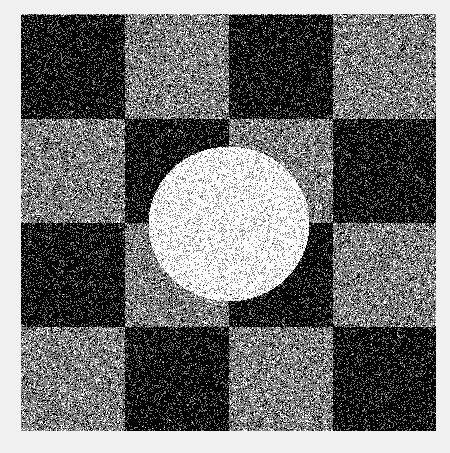
\includegraphics[scale=0.3]{Imgs/MRF_S1_Init.png}
	\caption{دسته‌بندی معمولی}
	\end{subfigure}
	\begin{subfigure}{0.4\textwidth}
	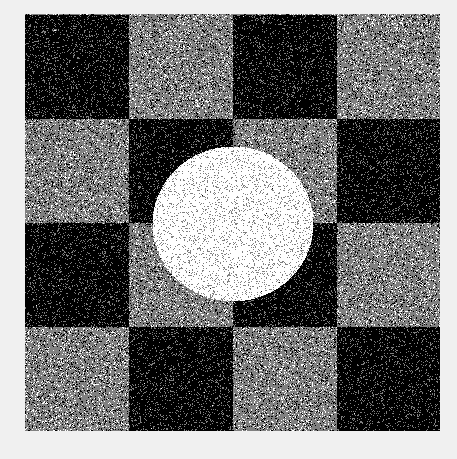
\includegraphics[scale=0.3]{Imgs/MRF_S1_BetaV_Res.png}
	\caption{دسته‌بندی با مقداردهی اولیه 5 درصد از نقاط}
	\end{subfigure}	
\caption{مقایسه تاثیر مقداردهی اولیه برخی نقاط. تصویر نویزی با $\sigma=0.1$}
\label{fig:Init}
\end{figure}


%%%%%%%%%%%%%%%%%%%%%%%%%%%%%%%%%%%%%%%%%%%%%%%%%%%%%%%%%%%%%%%%%%%%%%%%%%%%%%%%%%%
\subsection{تاثیر نوع همسایگی}

در صورتی‌که همسایگی نقاط را به شکل ۴ تایی در نظر بگیریم،‌ برچسب هر پیکسل فقط با همسایگان عمودی و افقی خود مقایسه می‌شود. این مساله می‌تواند باعث کاهش دقت الگوریتم و باقی‌ماندن نویزهای مورب در تصویر شود. اگر همسایگی نقاط را به شکل ۸ تایی درنظر بگیریم،‌ از آنجا که تعداد همسایگانی که برچسب هر پیکسل را با آن‌ها مقایسه ‌می‌کنیم افزایش می‌یابد،‌ دقت الگوریتم افزایش خواهد یافت. با درنظر داشتن بهبودی که در بخش «بررسی مدل» ارائه شد (محاسبه تغییرات تابع آرا به جای مقدار تابع در کل تصویر)،‌ افزایش تعداد همسایگی‌های مورد بررسی،‌ تاثیری در زمان اجرای الگوریتم نخواهد داشت.
\\
شکل 
\ref{fig:Neigh}
تاثیر نوع همسایگی را بر عملکرد الگوریتم نمایش می‌دهد.

\begin{figure}[h]
\center
	\begin{subfigure}{0.4\textwidth}
	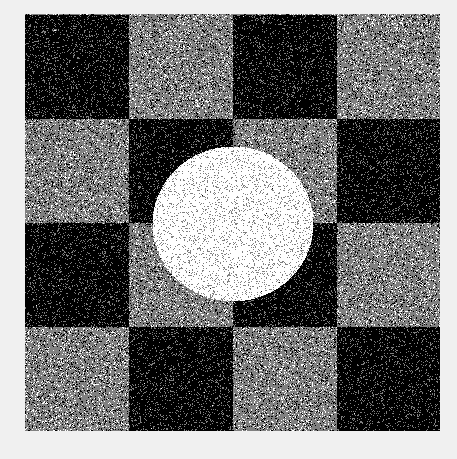
\includegraphics[scale=0.3]{Imgs/MRF_S1_BetaV_Res.png}
	\caption{همسایگی ۸ تایی}
	\end{subfigure}
	\begin{subfigure}{0.4\textwidth}
	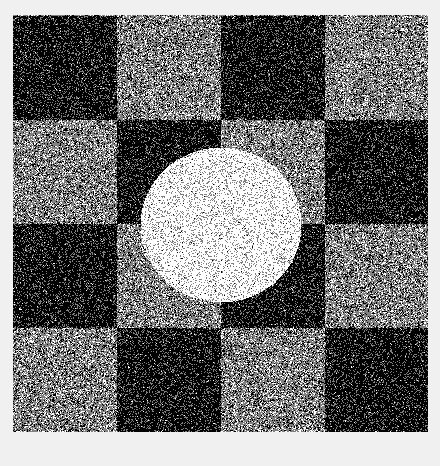
\includegraphics[scale=0.3]{Imgs/MRF_Neig4.png}
	\caption{همسایگی ۴ تایی}
	\end{subfigure}	
\caption{مقایسه تاثیر نوع همسایگی. تصویر نویزی با $\sigma=0.1$}
\label{fig:Neigh}
\end{figure}

%%%%%%%%%%%%%%%%%%%%%%%%%%%%%%%%%%%%%%%%%%%%%%%%%%%%%%%%%%%%%%%%%%%%%%%%%%%%%%%%%%%
\subsection{بررسی تاثیر نویز}
در دسته‌بندی‌کننده بیز ساده دیدیم افزایش قدرت نویز در تصویر می‌تواند باعث کاهش چشم‌گیر دقت فرایند تقطیع شود. در مدل میدان تصادفی مارکف، با اضافه کردن فاکتور یکپارچگی برچسب نقاط همسایه، تا حد خوبی این مشکل حل شد. اما در این مدل، اگر قدرت نویز زیاد باشد، تعداد تکرار بسیار بیشتری باید انجام شود تا به پاسخ بهینه دست‌پیدا کنیم. با این توضیح، انتظار داریم با افزایش قدرت نویز تصویر، تعداد مراحل مورد نیاز برای رسیدن به پاسخ نهایی افزایش یابد.
\\
شکل
\ref{fig:Noise}
تاثیر نویز را در عملکرد الگوریتم به نمایش گذاشته است. همان‌طور که مشاهده می‌شود، افزایش نویز تصویر، دقت تقطیع را کاهش می‌دهد.
\begin{figure}[h]
\center
	\begin{subfigure}{0.3\textwidth}
	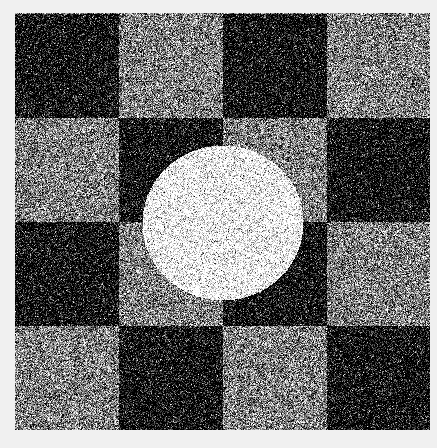
\includegraphics[scale=0.3]{Imgs/MRF_S1_In.png}
	\caption{تصویر نویزی با $\sigma=0.1$}
	\end{subfigure}
	\begin{subfigure}{0.3\textwidth}
	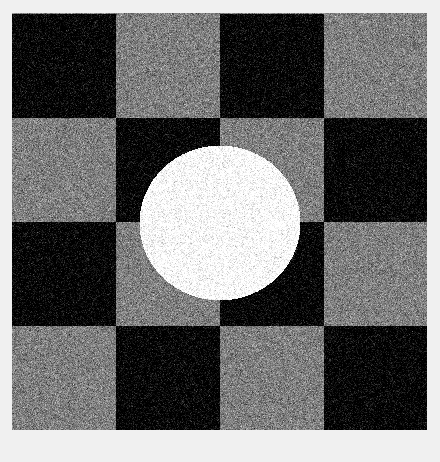
\includegraphics[scale=0.3]{Imgs/MRF_S01_In.png}
	\caption{تصویر نویزی با $\sigma=0.01$}
	\end{subfigure}	
	\begin{subfigure}{0.3\textwidth}
	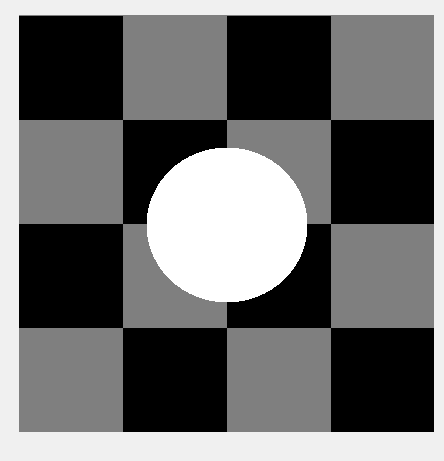
\includegraphics[scale=0.3]{Imgs/MRF_S0_In.png}
	\caption{تصویر بدون نویز}
	\end{subfigure}	

	\begin{subfigure}{0.3\textwidth}
	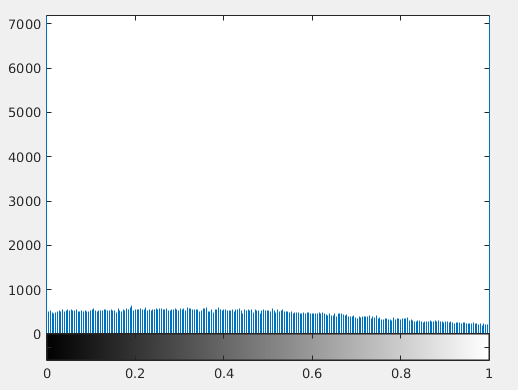
\includegraphics[scale=0.3]{Imgs/MRF_S1_Hist.png}
	\caption{هیستوگرام تصویر نویزی با $\sigma=0.1$}
	\end{subfigure}
	\begin{subfigure}{0.3\textwidth}
	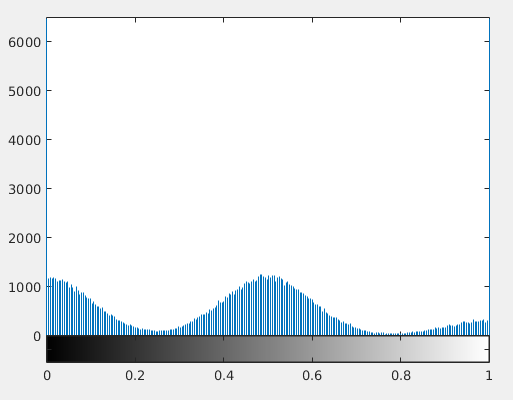
\includegraphics[scale=0.3]{Imgs/MRF_S01_Hist.png}
	\caption{هیستوگرام تصویر نویزی با $\sigma=0.01$}
	\end{subfigure}	
	\begin{subfigure}{0.3\textwidth}
	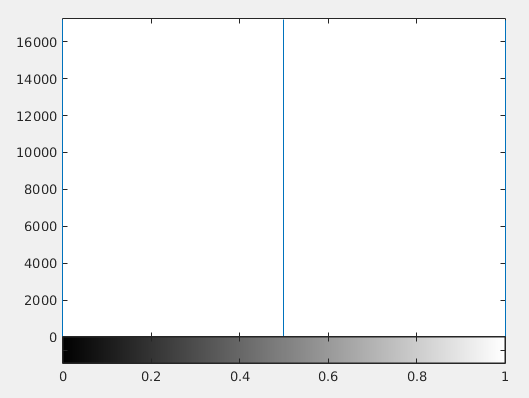
\includegraphics[scale=0.3]{Imgs/MRF_S0_Hist.png}
	\caption{هیستوگرام تصویر بدون نویز}
	\end{subfigure}	

	\begin{subfigure}{0.3\textwidth}
	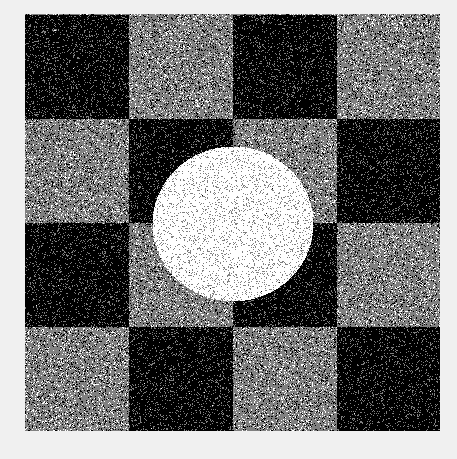
\includegraphics[scale=0.3]{Imgs/MRF_S1_BetaV_Res.png}
	\caption{خروجی الگوریتم برای تصویر نویزی با $\sigma=0.1$}
	\end{subfigure}
	\begin{subfigure}{0.3\textwidth}
	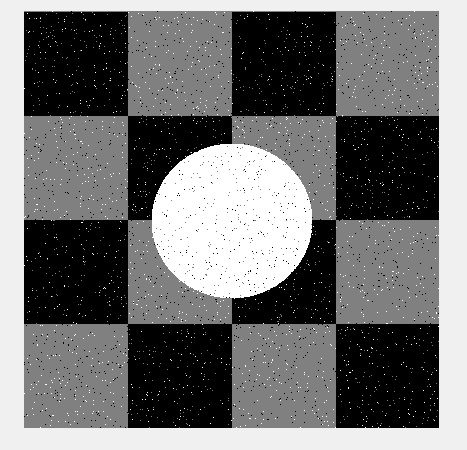
\includegraphics[scale=0.3]{Imgs/MRF_S01_Res.png}
	\caption{خروجی الگوریتم، تصویر نویزی با $\sigma=0.01$}
	\end{subfigure}	
	\begin{subfigure}{0.3\textwidth}
	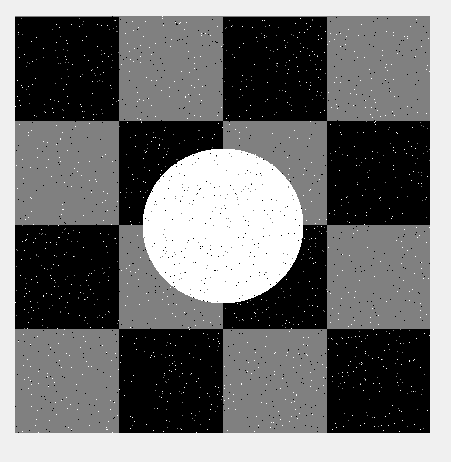
\includegraphics[scale=0.3]{Imgs/MRF_Iter4_TLin.png}
	\caption{خروجی الگوریتم برای تصویر نویزی با $\sigma=0$}
	\end{subfigure}	
\caption{مقایسه تاثیر نویز در عملکرد الگوریتم}
\label{fig:Noise}
\end{figure}


%%%%%%%%%%%%%%%%%%%%%%%%%%%%%%%%%%%%%%%%%%%%%%%%%%%%%%%%%%%%%%%%%%%%%%%%%%%%%%%%%%%
\subsection{تقطیع داده واقعی در فضاهای رنگی مختلف}
در این بخش از دو فضای رنگی مختلف برای تقطیع تصویر استفاده می‌نماییم. تصویر سطح خاکستری را مانند مثال‌های قبلی تقطیع می‌کنیم. برای پیدا کردن پارامترهای توزیع گاوسی برچسب‌ها در تصویر سطح خاکستری،‌ ابتدا هیستوگرام تصویر بدون نویز را بدست‌ می‌آوریم و سپس قله‌های هیستوگرام را به عنوان $\mu_i$ و نصف عرض هر قله را برابر با $\sigma_i$ قرار می‌دهیم. با بدست آوردن این اطلاعات، همانند مثال‌های قبلی، عمل تقطیع را انجام می‌دهیم.
\\
برای بررسی تاثیر فضاهای رنگی دیگر، فضای \lr{HSV} را به عنوان نمونه مورد بررسی قرار می‌دهیم. در این قسمت، ابتدا تصویر را از فضای رنگی به فضای \lr{HSV} منتقل کرده و سپس فاکتورهای \lr{SV} را فیلتر می‌کنیم. سپس تمام مراحل قبلی را روی تصویر بدست‌آمده اجرا می‌کنیم.
\\
شکل 
\ref{fig:HSV}
تاثیر فضاهای رنگی در دقت تقطیع را نمایش می‌دهد. در این شکل، خروجی الگوریتم به ازای دو نویز مختلف با قدرت‌های مختلف به نمایش گذاشته شده است. همان‌طور که مشاهده می‌شود، تقطیع در فضای رنگی \lr{HSV} دقت بیشتری دارد.
\begin{figure}[h]
\center
	\begin{subfigure}{0.4\textwidth}
	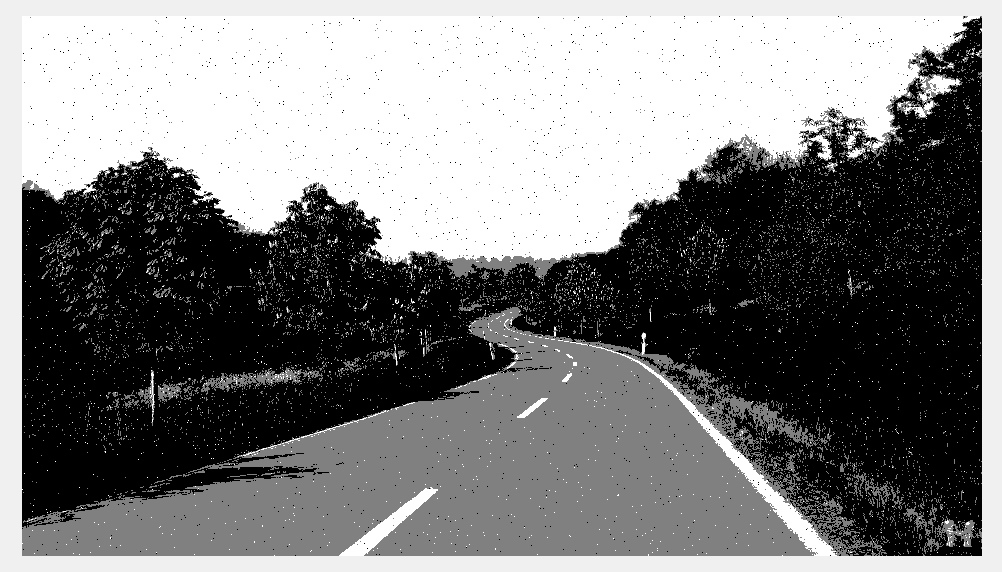
\includegraphics[scale=0.2]{Imgs/iter9_Gray_Classification.png}
	\caption{خروجی الگوریتم برای تصویر سطح خاکستری با $\sigma=0$}
	\end{subfigure}
	\begin{subfigure}{0.4\textwidth}
	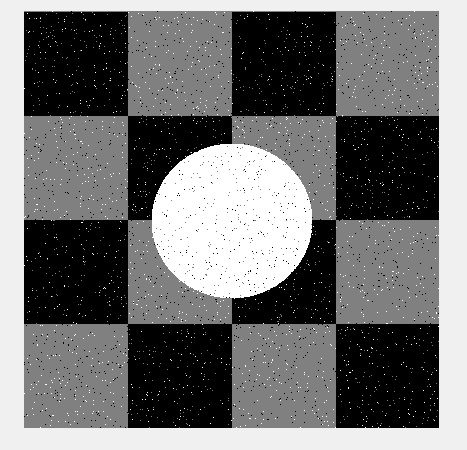
\includegraphics[scale=0.3]{Imgs/MRF_S01_Res.png}
	\caption{خروجی الگوریتم برای تصویر \lr{HSV} $\sigma=0$}
	\end{subfigure}	
	\begin{subfigure}{0.4\textwidth}
	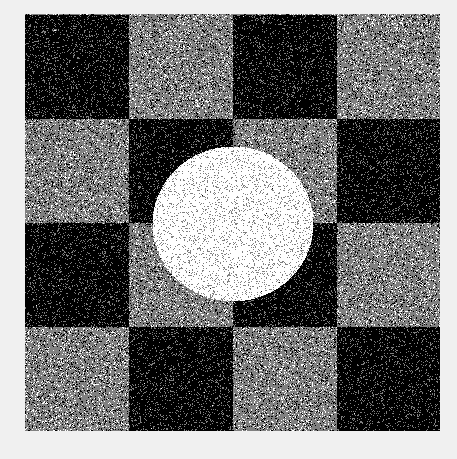
\includegraphics[scale=0.3]{Imgs/MRF_S1_BetaV_Res.png}
	\caption{خروجی الگوریتم برای تصویر سطح خاکستری با $\sigma=0.1$}
	\end{subfigure}
	\begin{subfigure}{0.4\textwidth}
	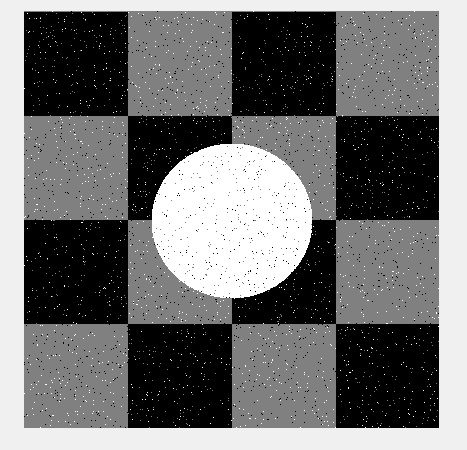
\includegraphics[scale=0.3]{Imgs/MRF_S01_Res.png}
	\caption{خروجی الگوریتم برای تصویر \lr{HSV} $\sigma=0.1$}
	\end{subfigure}	
\caption{مقایسه عملکرد الگوریتم در فضاهای رنگی مختلف}
\label{fig:HSV}
\end{figure}

 
%%%%%%%%%%%%%%%%%%%%%%%%%%%%%%%%%%%%%%%%%%%%%%%%%%%%%%%%%%%%%%%%%%%%%%%%%%%%%%%%%%%
\subsection{تقطیع تصویر با بیش از یک ویژگی}
در این قسمت برای استفاده از بیش از یک ویژگی در مدل، از هر دو ویژگی سطح خاکستری و پارامتر رنگی \lr{H} که در بخش قبلی مورد استفاده قرار گرفت، در تقطیع استفاده می‌کنیم. پارامترهای اولیه هر دو این ویژگی‌ها شامل $\mu$ و $\sigma$ قبلا محاسبه شده‌اند. فاکتور \lr{H} را به دو فاکتور موجود قبلی اضافه می‌نماییم و با بازنویسی رابطه 
\ref{eq:deltaV}
به بررسی نقش بیش از یک ویژگی در تصویر می‌پردازیم.
\\
شکل 
\ref{fig:MultFeat}
خروجی الگوریتم را در حالت تک ویژگی با استفاده از سطح خاکستری و در حالت دو ویژگی نمایش می‌دهد. همان‌طور که مشاهده می‌شود، خروجی الگوریتم در حالت دو ویژگی بهتر از حالت یک ‌ویژگی است.

\begin{figure}[h]
\center
	\begin{subfigure}{0.4\textwidth}
	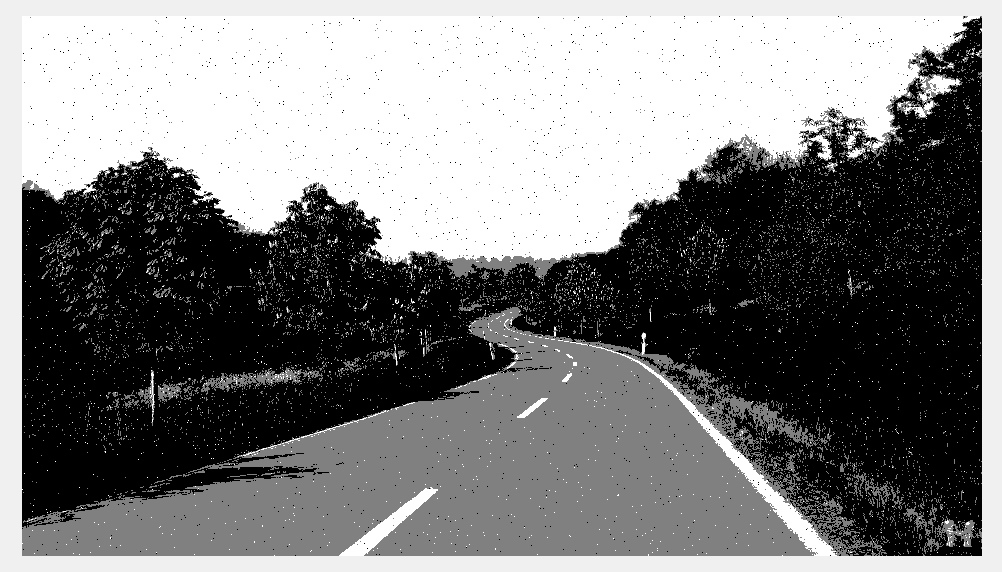
\includegraphics[scale=0.2]{Imgs/iter9_Gray_Classification.png}
	\caption{خروجی حالت سطح خاکستری}
	\end{subfigure}
	\begin{subfigure}{0.4\textwidth}
	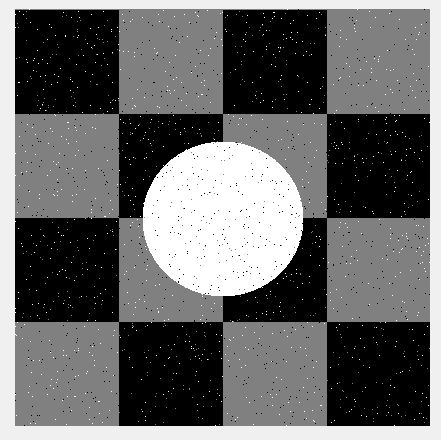
\includegraphics[scale=0.3]{Imgs/MRF_Iter4_TExp.png}
	\caption{خروجی حالت استفاده از بیش از یک ویژگی}
	\end{subfigure}	
\caption{مقایسه تاثیر استفاده بیش از یک ویژگی}
\label{fig:MultFeat}
\end{figure}


%%%%%%%%%%%%%%%%%%%%%%%%%%%%%%%%%%%%%%%%%%%%%%%%%%%%%%%%%%%%%%%%%%%%%%%%%%%%%%%%%%%
\vfill
\section{توضیحات}
\begin{itemize}
\item [*] با توجه به ز مان‌بر بودن اجرای کامل الگوریتم، عموم آزمایشات نتیجه تکرار چهارم و پنجم الگوریتم هستند. بدیهی  است ادامه اجرای الگوریتم بر بهبود پاسخ موثر خواهد بود اما نتایج مقایسات تغییری نخواهند کرد. 
\item [*] سورس کد مربوط به پروژه در ضمیمه این گزارش ارسال شده است. همین‌طور این کد از
\href{https://github.com/ahmad-asadi/PGM/tree/master/MarkovRandomField}
{این لینک}
، قابل 
دریافت می‌باشد.
%\item [*] آدرس لینک برای دریافت کد:
%\LTR{
%\url{https://github.com/ahmad-asadi/PGM/tree/master/BayesianNetwork}
%}
\end{itemize}




\end{document} 
